\phantomsection
\addcontentsline{toc}{part}{Appendix}
\phantomsection
\addchap{Language sample and maps} 
%%%

\section*{Taxon abbreviations (families)}
%%%
\begin{flushleft}
AB-AD=Abkhaz-Adyghe, AUA=Austroasiatic, AUN=Austronesian, C-SUD=Central Sudanic, CHAD=Chadic, CHAP=Chapacura-Wanham, CHU-K=Chukotko-Kamchatkan, CUSH=Cushitic, DRAV=Dravidian, ESK-A=Eskimo-Aleut, GUNW=Gunwingguan, HM-MI=Hmong-Mien, IE=Indo-European, IROQ=Iroquoian, KARTV=Kartvelian, KOIS=Koisan, KOM=Kombio, K-KRO=Kadugli-Krongo, MONG=Mongolic, MUSK=Muskogean, NA-DA=Nakh-Daghestanian, NA-DE=Na-Dene, NIG-C=Niger-Congo, NIL=Nilotic, S-BOU=South Bougainville, SE-RA=Lower Sepic-Ramu, SEM=Semitic, SIN-T=Sino-Tibetan, SONG=Songhai, TAI-K=Thai-Kadai, TANG=Tangkic, TNG=Trans New Guinea, TUNG=Tungusic, TURK=Turkic, U-AZT=Uto-Aztecan, URAL=Uralic, YEN=Yeniseian, YUK=Yukaghir
\end{flushleft}

\section*{Taxon abbreviations (branches and subbranches)}
%%%
\begin{flushleft}
5N=Five Nations, AAT=Avar-Andi-Tsezic, ABKH=Abkhaz, ALBA=Albanian, ALT=Altay, ARAM=Aramaic, ARAP=Arapesh, ARME=Armenian, ATHA=Athabaskan, ATLA=Atlantic, BALT=Baltic, BANT=Bantoid, BE-CO=Benue-Congo, BRIT=Brittonic, BULG=Bulgar, BURM=Burmic, CELT=Celtic, CH-IN=Chechen-Ingush, CHIN=Chinese, CHU=Chukotkan, CIRC=Circassian, COM=Common, DARG=Dargwa, ENE=Enets, ENIN=Enindhilyagwa, ESKI=Eskimo, DAGH=Daghestanian, DAG=Dagur, FINN=Finnic, FOR=Formosan, GAE=Gaelic, GEOR=Georgian, GER=Germanic, GREE=Greek, HAUS=Hausa, HELL=Hellenic, HMON=Hmongic, HUNG=Hungarian, I-ARY=Indo-Aryan, I-IRA=Indo-Iranian, IRAN=Iranian, IT-W=Italo-Western, KAMCH=Kamchatkan, KARL=Karluk, KHAN=Khanty, KHOE=Khoekhoe, KIPCH=Kipchak, KIRA=Kiranti, KORAL=Koryak-Alutor, KRON=Krongo, L-BUR=Lolo-Burmese, L-SEP-Lower Sepik, LEZG=Lezgic, LEND=Lendu, M-KH=Mon-Khmer, MADA=Madang, MAL-P=Malayo-Polynesian, MANCH=Manchu, MAND=Mande, MANS=Mansi, MOGH=Moghol, MONGO=Mongolian, MONGU=Monguor, MORD=Mordvin, NASI=Nasioi, NOU=Nanay-Orok-Ulcha, NENE=Nenets, NGAN=Nganasan, OCE=Oceanic, OR-UD=Oroch-Udege, OROM=Oromo, PERM=Permic,  REMB=Rembargic, ROM=Romance, S-WEL=South Wellesley, SAAM=Saamic, SAMO=Samoyedic, SAY=Sayan, SELK=Selkup, SIN=Sinitic, SLAV=Slavic, SUND=Sundic, TSO=Tsouic, VIET=Vietic, W-MP=Western Malayo-Polynesian, YEN=Yenisey, YI-KA=Yimas-Karawari, YOR=Yoruboid, YUP=Yupik
\end{flushleft}

\section*{Geographic (sample) abbreviations}
%%%
\begin{flushleft}
EU=\isi{Europe}, NA=\isi{North Asia}, NE=North Eurasia, W=World
\end{flushleft}

\is{juxtaposition|(}
\is{incorporation|(}
\is{construct state|(}
\is{anti\hyp{}construct state|(}
\is{attributive nominalization|(}
\is{attributive article|(}
\is{anti\hyp{}construct state agreement|(}
\is{head\hyp{}driven agreement|(}
\is{appositional head\hyp{}driven agreement|(}
\is{modifier\hyp{}headed possessor agreement|(}
\is{linker|(}

\section*{Type abbreviations}
%%%
\begin{flushleft}
ACAgr=Anti\hyp{}construct state agreement, AConstr=Anti\hyp{}construct state, AHDAgr=Appositional head\hyp{}driven agreement, Constr=Construct state, DConstr=Double\hyp{}construct state, HDAgr=Head\hyp{}driven agreement, Inc=Adjective incorporation, Juxt=Juxtaposition, Link=Linker, MHPAgr=Modifier\hyp{}headed possessor agreement, Nmlz=Attributive nominalization
\end{flushleft}

\begin{sidewaystable}
\resizebox{.9\textwidth}{!}{
\begin{tabular}{llllcccclp{5.5cm}}\label{sample8}
\\%LATEX does not compile without this empty line
\lsptoprule
\multicolumn{4}{c}{Genealogical affiliation}&\multicolumn{4}{c}{Geographic sampling}&Noun phrase type(s)&\\\cmidrule(lr){1-4}\cmidrule(lr){5-8}%\cmidrule(lr){9-9}
%\hline%\midrule
Family&\multicolumn{2}{l}{(Sub-)Branch}&Language &EU&NA&NE&W &\#1/\#2(\#3)[\#4]&Reference\\
\midrule
\multicolumn{3}{l}{	(Pidgin and creoles)	}					&	\textsc{	Berbice Dutch Creole	}	&	–	&	–	&	–	&	X	&	Juxt	&	\citealt{kouwenberg1994}\il{Berbice Dutch Creole}\\
{	AB-AD	}	&	ABKH	&		&	\textsc{	Abaza	}	&	X	&	–	&	–	&	–	&	HDAgr	&	\citealt{lomtatidze-etal1989}\il{Abaza}\\
{	AB-AD	}	&	ABKH	&		&	\textsc{	Abkhaz	}	&	X	&	–	&	X	&	X	&	HDAgr	&	\citealt{chirikba2003}	\il{Abkhaz}\\
{	AB-AD	}	&	CIRC	&		&	\textsc{	Adyghe (Abzakh)	}	&	X	&	–	&	–	&	–	&	Inc	&	\citealt{paris1989}\il{Adyghe!Abzakh}\\
{	AB-AD	}	&	CIRC	&		&	\textsc{	Karbardian	}	&	X	&	–	&	X	&	–	&	Inc	&	\citealt{colarusso2006}\il{Karbardian}\\
\multicolumn{3}{l}{	AINU (isolate)	}					&	\textsc{	Ainu	}	&	–	&	X	&	X	&	X	&	Juxt	&	\citealt{refsing1986}\il{Ainu}\\
{	AUA	}	&	M-KH	&	VIET	&	\textsc{	Vietnamese	}	&	–	&	–	&	–	&	X	&	Juxt	&	\citealt{nguyen1987}\il{Vietnamese}\\
{	AUN	}	&	FOR	&	TSO	&	\textsc{	Tsou	}	&	–	&	–	&	–	&	X	&	AConstr	&	\citealt{szakos1994}\il{Tsou}\\
{	AUN	}	&	MAL-P	&	OCE	&	\textsc{	Saliba	}	&	–	&	–	&	–	&	X	&	MHPAgr	&	\citealt{mosel1994}\il{Saliba}\\
{	AUN	}	&	MAL-P	&	OCE	&	\textsc{	Takia	}	&	–	&	–	&	–	&	X	&	AConstr	&	\citealt{ross1998}\il{Takia}\\
{	AUN	}	&	WEMP	&	M-PH	&	\textsc{	Tagalog	}	&	–	&	–	&	–	&	X	&	Linker	&	\citealt{schachter1987}\il{Tagalog}\\
{	AUN	}	&	WEMP	&	SUND	&	\textsc{	Minangkabau	}	&	–	&	–	&	–	&	–	&	Juxt	&	\citealt{gil2005}\il{Minangkabau}\\
\multicolumn{3}{l}{	BASQUE (isolate)	}					&	\textsc{	Basque	}	&	X	&	–	&	X	&	X	&	Juxt	&	\citealt{hualde-etal2003}\il{Basque}\\
{	C-SUD	}	&	E	&	LEND	&	\textsc{	Ngiti	}	&	–	&	–	&	–	&	X	&	HDAgr/Juxt	&	\citealt{kutsch-lojenga1994}\il{Ngiti}\\
\multicolumn{3}{l}{	CARIBAN	}					&	\textsc{	Hixkaryana	}	&	–	&	–	&	–	&	X	&	n.a.	&	\citealt{derbyshire1979}\il{Hixkaryana}\\
{	CHAD	}	&	W	&	HAUS	&	\textsc{	Hausa	}	&	–	&	–	&	–	&	X	&	ACAgr/HDAgr	&	\citealt{wolff1993}\il{Hausa}\\
{	CHAP	}	&		&		&	\textsc{	Wari'	}	&	–	&	–	&	–	&	X	&	MHPAgr	&	\citealt{everett-etal1997}\il{Wari'}\\
{	CHU-K	}	&	CHU	&		&	\textsc{	Chukchi	}		&	–	&	X	&	X	&	X	&	Inc/HDAgr	&	\citealt{skorik1960}\il{Chukchi}\\
{	CHU-K	}	&	CHU	&	KORAL	&	\textsc{	Alutor	}	&	–	&	X	&	–	&	–	&	Inc/HDAgr	&	\citealt{nagayama2003}\il{Alutor}\\
{	CHU-K	}	&	CHU	&	KORAL	&	\textsc{	Koryak	}	&	–	&	X	&	X	&	–	&	Inc	&	\citealt{zukova1997}\il{Koryak}\\
{	CHU-K	}	&	KAMCH	&	W	&	\textsc{	Itelmen	}	&	–	&	X	&	X	&	–	&	ACAgr	&	\citealt{georg-etal1999}\il{Itelmen}\\
{	CUSH	}	&	E	&	OROM	&	\textsc{	Oromo (Boraana)	}	&	–	&	–	&	–	&	X	&	HDAgr	&	\citealt{stroomer1995}\il{Oromo!Boraana}\\
{	DRAV	}	&	S	&		&	\textsc{	Tamil	}	&	–	&	–	&	–	&	X	&	Juxt	&	\citealt{asher1982}\il{Tamil}\\
{	ESK-A	}	&	ESKI	&	YUP	&	\textsc{	Yupik (Siberian)	}	&	–	&	X	&	X	&	–	&	Inc	&	\citealt{de-reuse1994}\il{Central Siberian Yupik}\\
{	ESK-A	}	&	ESKI	&		&	\textsc{	Western Greenlandic	}	&	–	&	–	&	–	&	X	&	HDAgr	&	\citealt{fortescue1984}\il{Western Greenlandic}\\
{	GUNW	}	&	REMB	&		&	\textsc{	Ngalakan	}	&	–	&	–	&	–	&	X	&	HDAgr/Juxt	&	\citealt{merlan1983}\il{Ngalakan}\\
{	HM-MI	}	&	HMON	&		&	\textsc{	Hmong Njua	}	&	–	&	–	&	–	&	X	&	Juxt	&	\citealt{harriehausen1990}\il{Hmong Njua}\\
{	IE	}	&	ALBA	&		&	\textsc{	Albanian	}	&	X	&	–	&	X	&	X	&	HDAgr/Nmlz+HDAgr	&	\citealt{demiraj1998}\il{Albanian}\\
{	IE	}	&	ALBA	&		&	\textsc{	Arvanitika	}	&	X	&	–	&	–	&	–	&	HDAgr/Nmlz+HDAgr	&	\citealt{sasse1991}\il{Arvanitika}\\
{	IE	}	&	ARME	&		&	\textsc{	Armenian (Eastern)	}	&	X	&	–	&	X	&	–	&	HDAgr/Juxt	&	\citealt{ajello1998}\il{Eastern Armenian}\\
\lspbottomrule
\end{tabular}
}
%\end{footnotesize}
\end{sidewaystable}

\begin{sidewaystable}
\resizebox{.9\textwidth}{!}{
\begin{tabular}{llllcccclp{5.5cm}}\label{sample1}
\\%LATEX does not compile without this empty line
\lsptoprule
\multicolumn{4}{c}{Genealogical affiliation}&\multicolumn{4}{c}{Geographic sampling}&Noun phrase type(s)&\\\cmidrule(lr){1-4}\cmidrule(lr){5-8}%\cmidrule(lr){9-9}
%\hline%\midrule
Family&\multicolumn{2}{l}{(Sub-)Branch}&Language &EU&NA&NE&W &\#1/\#2(\#3)[\#4]&Reference\\
\midrule
{	IE	}	&	BALT	&	E	&	\textsc{	Latvian	}	&	X	&	–	&	X	&	–	&	ACAgr/HDAgr	&	\citealt{nau1996}\il{Latvian}\\
{	IE	}	&	BALT	&	E	&	\textsc{	Lithuanian	}	&	X	&	–	&	–	&	–	&	ACAgr/HDAgr	&	\citealt{press2005}\il{Lithuanian}\\
{	IE	}	&	CELT	&	BRIT	&	\textsc{	Breton	}	&	X	&	–	&	–	&	–	&	HDAgr	&	
\citealt{ternes1992}\il{Breton}\\
{	IE	}	&	CELT	&	BRIT	&	\textsc{	Cornish	}	&	X	&	–	&	–	&	–	&	HDAgr	&	\citealt{thomas1992b}\il{Cornish}\\
{	IE	}	&	CELT	&	BRIT	&	\textsc{	Welsh	}	&	X	&	–	&	X	&	–	&	HDAgr	&	\citealt{thomas1992a}\il{Welsh}\\
{	IE	}	&	CELT	&	GAE	&	\textsc{	Gaelic (Scots)	}	&	X	&	–	&	X	&	–	&	HDAgr	&	\citealt{macauley1992}\il{Scots Gaelic}\\
{	IE	}	&	CELT	&	GAE	&	\textsc{	Irish	}	&	X	&	–	&	–	&	–	&	HDAgr	&	\citealt{odochartaigh1992}\il{Irish}\\
{	IE	}	&	CELT	&	GAE	&	\textsc{	Manx	}	&	X	&	–	&	X	&	–	&	HDAgr/Juxt	&	\citealt{phillips2004}\il{Manx}\\
{	IE	}	&	GER	&	N	&	\textsc{	Danish	}	&	X	&	–	&	–	&	–	&	HDAgr[Nmlz]	&	own knowledge\il{Danish}\\
{	IE	}	&	GER	&	N	&	\textsc{	Danish (W-Jutlandic)	}	&	–	&	–	&	–	&	–	&	HDAgr	&	\citealt{lund1932}\il{Danish!W-Jutlandic}\\
{	IE	}	&	GER	&	N	&	\textsc{	Faroese	}	&	X	&	–	&	–	&	–	&	ACAgr+HDAgr/HDAgr[Nmlz]	&	\citealt{lockwood1955}\il{Faroese}\\
{	IE	}	&	GER	&	N	&	\textsc{	Icelandic	}	&	X	&	–	&	X	&	–	&	HDAgr[Nmlz]	&	\citealt{kress1982}\il{Icelandic}\\
{	IE	}	&	GER	&	N	&	\textsc{	Norwegian	}	&	X	&	–	&	–	&	–	&	ACAgr+HDAgr/HDAgr[Nmlz]	&	own knowledge\il{Norwegian}\\
{	IE	}	&	GER	&	N	&	\textsc{	Swedish	}	&	X	&	–	&	X	&	–	&	ACAgr+HDAgr/HDAgr[Nmlz]	&	own knowledge	\il{Swedish}\\
{	IE	}	&	GER	&	N	&	\textsc{	Swedish (Västerbotten)	}	&	X	&	–	&	X	&	–	&	Inc/HDAgr	&	\citealt{astrom1893}\il{Swedish!Västerbotten}\\
{	IE	}	&	GER	&	W	&	\textsc{	Dutch	}	&	X	&	–	&	–	&	–	&	ACAgr[Nmlz]	&	\citealt{donaldson1997}\il{Dutch}\\
{	IE	}	&	GER	&	W	&	\textsc{	English	}	&	X	&	–	&	X	&	X	&	Inc[Nmlz]	&	own knowledge\il{English}\\
{	IE	}	&	GER	&	W	&	\textsc{	Frisian (West)	}	&	X	&	–	&	–	&	–	&	ACAgr	&	\citealt{tiersma1985}\il{Western Frisian}\\
{	IE	}	&	GER	&	W	&	\textsc{	German	}	&	X	&	–	&	X	&	–	&	ACAgr[Nmlz]	&	own knowledge\il{German}\\
{	IE	}	&	GER	&	W	&	\textsc{	German (Alemannic)	}	&	X	&	–	&	–	&	–	&	ACAgr	&	\citealt{reese2006}\il{Alemannic}\\
{	IE	}	&	GER	&	W	&	\textsc{	German (Low)	}	&	X	&	–	&	–	&	–	&	ACAgr	&	\citealt{matras-etal2003}\il{Lower German}\\
{	IE	}	&	GER	&	W	&	\textsc{	Luxembourgeois	}	&	X	&	–	&	–	&	–	&	ACAgr	&	\citealt{schanen-etal2006}\il{Luxembourgeois}\\
{	IE	}	&	GER	&	W	&	\textsc{	Yiddish (East)	}	&	X	&	–	&	–	&	–	&	ACAgr(Nmlz+HDAgr)	&	\citealt{katz1987}\il{Yiddish!Eastern}\\
{	IE	}	&	HELL	&	GREE	&	\textsc{	Greek	}	&	X	&	–	&	X	&	X	&	HDAgr(Nmlz+HDAgr)	&	\citealt{ruge1986}\il{Greek}\\
{	IE	}	&	I-IRA	&	I-ARY	&	\textsc{	Palula	}	&	–	&	X	&	X	&	–	&	HDAgr[Juxt]	&	\citealt{liljegren2016a}\il{Palula}\\
{	IE	}	&	I-IRA	&	I-ARY	&	\textsc{	Parya	}	&	–	&	X	&	X	&	–	&	ACAgr/Juxt	&	\citealt{oranskaja2001}\il{Parya}\\
{	IE	}	&	I-IRA	&	I-ARY	&	\textsc{	Romani (Burgenland)	}	&	X	&	–	&	X	&	–	&	HDAgr(Nmlz+HDAgr)	&	\citealt{halwachs-etal2002}\il{Romani!Burgenland}\\
{	IE	}	&	I-IRA	&	I-ARY	&	\textsc{	Romani (Doplenjska)	}	&	X	&	–	&	–	&	–	&	HDAgr	&	\citealt{cech2006}\il{Romani!Doplenjska}\\
{	IE	}	&	I-IRA	&	I-ARY	&	\textsc{	Romani (Lithuanian)	}	&	X	&	–	&	–	&	–	&	HDAgr	&	\citealt{tenser2005}\il{Romani!Lithuanian}\\
{	IE	}	&	I-IRA	&	I-ARY	&	\textsc{	Romani (Sepečides)	}	&	X	&	–	&	–	&	–	&	HDAgr	&	\citealt{cech-etal2003}\il{Romani!Sepečides}\\
\lspbottomrule
\end{tabular}
}
%\end{footnotesize}
\end{sidewaystable}
\begin{sidewaystable}
\resizebox{.9\textwidth}{!}{
		\begin{tabular}{llllcccclp{5.5cm}}\label{sample2}
			\\%LATEX does not compile without this empty line
			\lsptoprule
			\multicolumn{4}{c}{Genealogical affiliation}&\multicolumn{4}{c}{Geographic sampling}&Noun phrase type(s)&\\\cmidrule(lr){1-4}\cmidrule(lr){5-8}%\cmidrule(lr){9-9}
			%\hline%\midrule
			Family&\multicolumn{2}{l}{(Sub-)Branch}&Language &EU&NA&NE&W &\#1/\#2(\#3)[\#4]&Reference\\
			\midrule
{	IE	}	&	I-IRA	&	I-ARY	&	\textsc{	Romani (Sinte)	}	&	X	&	–	&	–	&	–	&	HDAgr	&	\citealt{holzinger1995}\il{Romani!Sinte}\\
{	IE	}	&	I-IRA	&	IRAN	&	\textsc{	Kurdish (Northern)}	&	X	&	–	&	–	&	–	&	Constr	&	\citealt{aygen2007}\il{Northern Kurdish}\\
{	IE	}	&	I-IRA	&	IRAN	&	\textsc{	Ossetic	}	&	X	&	–	&	X	&	–	&	Juxt(Constr)	&	\citealt{abaev1964}\il{Ossetic}\\
{	IE	}	&	I-IRA	&	IRAN	&	\textsc{	Persian	}	&	–	&	–	&	–	&	X	&	Constr	&	\citealt{mahootian1997}\il{Persian}\\
{	IE	}	&	I-IRA	&	IRAN	&	\textsc{	Rushani	}	&	–	&	X	&	–	&	–	&	AConstr(Constr)	&	\citealt{payne1989}\il{Rushani}\\
{	IE	}	&	I-IRA	&	IRAN	&	\textsc{	Shughni	}	&	–	&	X	&	–	&	–	&	HDAgr	&	\citealt{payne1989}\il{Shughni}\\
{	IE	}	&	I-IRA	&	IRAN	&	\textsc{	Tajik	}	&	–	&	X	&	X	&	–	&	Constr	&	\citealt{ido2005}\il{Tajik}\\
{	IE	}	&	I-IRA	&	IRAN	&	\textsc{	Talysh (Northern)	}	&	X	&	–	&	X	&	–	&	AConstr	&	\citealt{schulze2000}\il{Northern Talysh}\\
{	IE	}	&	I-IRA	&	IRAN	&	\textsc{	Tati	}	&	X	&	–	&	–	&	–	&	Constr	&	\citealt{dzidalaev2000}\il{Tati}\\
{	IE	}	&	I-IRA	&	IRAN	&	\textsc{	Yazghulami	}	&	–	&	X	&	X	&	–	&	HDAgr	&	\citealt{payne1989}\il{Yazghulami}\\
{	IE	}	&	ROM	&	E	&	\textsc{	Romanian	}	&	X	&	–	&	X	&	–	&	HDAgr(Nmlz+HDAgr)	&	\citealt{beyer-etal1987}\il{Romanian}\\
{	IE	}	&	ROM	&	IT-W	&	\textsc{	French	}	&	X	&	–	&	–	&	–	&	HDAgr	&	\citealt{harris1997}\il{French}\\
{	IE	}	&	ROM	&	IT-W	&	\textsc{	Galician	}	&	X	&	–	&	–	&	–	&	HDAgr	&	\citealt{perez-bouza1996}\il{Galician}\\
{	IE	}	&	ROM	&	IT-W	&	\textsc{	Italian	}	&	X	&	–	&	X	&	X	&	HDAgr	&	\citealt{maiden-etal2000}\il{Italian}\\
{	IE	}	&	ROM	&	IT-W	&	\textsc{	Portuguese	}	&	X	&	–	&	–	&	–	&	HDAgr	&	\citealt{gartner1998}\il{Portuguese}\\
{	IE	}	&	ROM	&	IT-W	&	\textsc{	Romansch	}	&	X	&	–	&	–	&	–	&	HDAgr	&	\citealt{haiman1997}\il{Romansch}\\
{	IE	}	&	ROM	&	IT-W	&	\textsc{	Spanish (Castilian)	}	&	X	&	–	&	–	&	–	&	HDAgr	&	\citealt{torrego1998}\il{Castilian}\\
{	IE	}	&	ROM	&	IT-W	&	\textsc{	Spanish (Catalan)	}	&	X	&	–	&	–	&	–	&	HDAgr	&	\citealt{hualde1992}\il{Catalan}\\
{	IE	}	&	ROM	&	S	&	\textsc{	Corsican	}	&	X	&	–	&	–	&	–	&	HDAgr	&	\citealt{giacomo-marcellesi1997}\il{Corsican}\\
{	IE	}	&	ROM	&	S	&	\textsc{	Sardinian	}	&	X	&	–	&	X	&	–	&	HDAgr	&	\citealt{jones1997}\il{Sardinian}\\
{	IE	}	&	SLAV	&	E	&	\textsc{	Belorussian	}	&	X	&	–	&	–	&	–	&	HDAgr	&	\citealt{mayo1993}\il{Belorussian}\\
{	IE	}	&	SLAV	&	E	&	\textsc{	Russian	}	&	X	&	–	&	X	&	X	&	ACAgr	&	own knowledge\il{Russian}\\
{	IE	}	&	SLAV	&	E	&	\textsc{	Ukrainian	}	&	X	&	–	&	X	&	–	&	HDAgr	&	\citealt{shevelov1993}\il{Ukrainian}\\
{	IE	}	&	SLAV	&	S	&	\textsc{	Bulgarian	}	&	X	&	–	&	X	&	–	&	HDAgr	&	own knowledge\il{Bulgarian}\\
{	IE	}	&	SLAV	&	S	&	\textsc{	Macedonian	}	&	X	&	–	&	–	&	–	&	HDAgr	&	\citealt{friedman2002}\il{Macedonian}\\
{	IE	}	&	SLAV	&	S	&	\textsc{	Serbo-Croatian	}	&	X	&	–	&	–	&	–	&	HDAgr(ACAgr)	&	\citealt{kordic1997}\il{Serbo-Croatian}\\
{	IE	}	&	SLAV	&	S	&	\textsc{	Slovenian	}	&	X	&	–	&	–	&	–	&	HDAgr(ACAgr)[Nmlz+HDAgr]	&	\citealt{priestly1993}\il{Slovenian}\\
{	IE	}	&	SLAV	&	W	&	\textsc{	Czech	}	&	X	&	–	&	–	&	–	&	HDAgr	&	\citealt{janda-etal2000}\il{Czech}\\
{	IE	}	&	SLAV	&	W	&	\textsc{	Kashubian	}	&	X	&	–	&	–	&	–	&	HDAgr	&	\citealt{stone1993b}\il{Kashubian}\\
{	IE	}	&	SLAV	&	W	&	\textsc{	Polish	}	&	X	&	–	&	–	&	–	&	HDAgr	&	\citealt{feldstein-etal2002}\il{Polish}\\
\lspbottomrule
\end{tabular}
}
%\end{footnotesize}
\end{sidewaystable}

\begin{sidewaystable}
\resizebox{.9\textwidth}{!}{
		\begin{tabular}{llllcccclp{5.5cm}}\label{sample3}
			\\%LATEX does not compile without this empty line
			\lsptoprule
			\multicolumn{4}{c}{Genealogical affiliation}&\multicolumn{4}{c}{Geographic sampling}&Noun phrase type(s)&\\\cmidrule(lr){1-4}\cmidrule(lr){5-8}%\cmidrule(lr){9-9}
			%\hline%\midrule
			Family&\multicolumn{2}{l}{(Sub-)Branch}&Language &EU&NA&NE&W &\#1/\#2(\#3)[\#4]&Reference\\
			\midrule

{	IE	}	&	SLAV	&	W	&	\textsc{	Slovak	}	&	X	&	–	&	–	&	–	&	HDAgr	&	\citealt{short1993b}\il{Slovak}\\
{	IE	}	&	SLAV	&	W	&	\textsc{	Sorbian (Lower)	}	&	X	&	–	&	X	&	–	&	HDAgr	&	\citealt{stone1993a}\il{Lower Sorbian}\\
{	IE	}	&	SLAV	&	W	&	\textsc{	Sorbian (Upper)	}	&	X	&	–	&	–	&	–	&	HDAgr	&	\citealt{schaarschmidt2004}\il{Upper Sorbian}\\
{	IROQ	}	&	N	&	5N	&	\textsc{	Cayuga	}	&	–	&	–	&	–	&	X	&	Inc	&	\citealt{mithun-etal1982}\il{Cayuga}\\
\multicolumn{3}{l}{	JAPANESE (isolate)	}					&	\textsc{	Japanese	}	&	–	&	X	&	X	&	X	&	AConstr/Juxt	&	\citealt{backhouse1984}\il{Japanese}\\
{	K-KRO	}	&	KRON	&		&	\textsc{	Krongo	}	&	–	&	–	&	–	&	X	&	ACAgr	&	\citealt{reh1985}\il{Krongo}\\
{	KARTV	}	&	GEOR	&		&	\textsc{	Georgian	}	&	X	&	–	&	X	&	X	&	HDAgr/Juxt(AHDAgr)	&	\citealt{cherchi1999}\il{Georgian}\\
{	KARTV	}	&	SVAN	&		&	\textsc{	Svan	}	&	X	&	–	&	X	&	–	&	HDAgr[Juxt]	&	\citealt{schmidt1991}\il{Svan}\\
{	KARTV	}	&	ZAN	&		&	\textsc{	Laz	}	&	X	&	–	&	X	&	–	&	Juxt(HDAgr)	&	\citealt{holisky1991}\il{Laz}\\
{	KARTV	}	&	ZAN	&		&	\textsc{	Mingrelian	}	&	X	&	–	&	–	&	–	&	Juxt(HDAgr)	&	\citealt{harris1991b}\il{Mingrelian}\\
{	KOIS	}	&	C	&	KHOE	&	\textsc{	Nama	}	&	–	&	–	&	–	&	X	&	Juxt	&	\citealt{hagman1977}\il{Nama}\\
{	KOM	}	&	ARAP	&		&	\textsc{	Arapesh (Bukiyip)	}	&	–	&	–	&	–	&	X	&	Juxt	&	\citealt{conrad1991}\il{Arapesh!Bukiyip}\\
\multicolumn{3}{l}{	KOREAN (isolate)	}					&	\textsc{	Korean	}	&	–	&	X	&	X	&	X	&	AConstr	&	\citealt{martin-etal1969}\il{Korean}\\
\multicolumn{3}{l}{	MAPUDUNGUN (isolate)	}					&	\textsc{	Mapudungun	}	&	–	&	–	&	–	&	X	&	ACAgr/Juxt	&	\citealt{zuniga2000}\il{Mapudungun}\\
{	MONG	}	&	DAG	&		&	\textsc{	Dagur	}	&	–	&	X	&	X	&	–	&	Juxt	&	\citealt{tsumagari2003}\il{Dagur}\\
{	MONG	}	&	MOGH	&		&	\textsc{	Moghol	}	&	–	&	X	&	–	&	X	&	Juxt	&	\citealt{weiers2003}\il{Moghol}\\
{	MONG	}	&	MONGO	&		&	\textsc{	Buryat	}	&	–	&	X	&	–	&	–	&	Juxt	&	\citealt{skribnik2003}\il{Buryat}\\
{	MONG	}	&	MONGO	&		&	\textsc{	Kalmyk	}	&	–	&	X	&	–	&	–	&	Juxt	&	\citealt{blasing2003}\il{Kalmyk}\\
{	MONG	}	&	MONGO	&		&	\textsc{	Khalkha	}	&	–	&	X	&	X	&	X	&	Juxt	&	\citealt{svantesson2003}\il{Khalkha}\\
{	MONG	}	&	MONGO	&		&	\textsc{	Mongol (Khamnigan)	}	&	–	&	X	&	–	&	–	&	Juxt	&	\citealt{janhunen2005}\il{Mongol!Khamnigan}\\
{	MONG	}	&	MONGO	&		&	\textsc{	Oyrat	}	&	–	&	–	&	–	&	–	&	Juxt	&	\citealt{birtalan2003}\il{Oyrat}\\
{	MONG	}	&	MONGU	&		&	\textsc{	Mangghuer	}	&	–	&	–	&	–	&	–	&	Juxt	&	\citealt{slater2003}\il{Mangghuer}\\
{	MUSK	}	&	E	&		&	\textsc{	Koasati	}	&	–	&	–	&	–	&	X	&	Nmlz	&	\citealt{kimball1991}\il{Koasati}\\
{	NA-DA	}	&	DAGH	&	AAT	&	\textsc{	Akhvakh	}	&	X	&	–	&	–	&	–	&	HDAgr	&	\citealt{magomedbekova2000}\il{Akhvakh}\\
{	NA-DA	}	&	DAGH	&	AAT	&	\textsc{	Andi	}	&	X	&	–	&	–	&	–	&	HDAgr	&	\citealt{saidova2000}\il{Andi}\\
{	NA-DA	}	&	DAGH	&	AAT	&	\textsc{	Avar	}	&	X	&	–	&	–	&	X	&	HDAgr(Juxt)	&	\citealt{alekseev-etal1997}\il{Avar}\\
{	NA-DA	}	&	DAGH	&	AAT	&	\textsc{	Bagvalal	}	&	X	&	–	&	–	&	–	&	HDAgr	&	\citealt{magomedova2000a}\il{Bagvalal}\\
{	NA-DA	}	&	DAGH	&	AAT	&	\textsc{	Bezhta	}	&	X	&	–	&	–	&	–	&	HDAgr	&	\citealt{KibrikEtAl2004}\il{Bezhta}\\
{	NA-DA	}	&	DAGH	&	AAT	&	\textsc{	Botlikh	}	&	–	&	–	&	–	&	–	&	HDAgr	&	\citealt{azaev2000}\il{Botlikh}\\
{	NA-DA	}	&	DAGH	&	AAT	&	\textsc{	Chamalal	}	&	X	&	–	&	–	&	–	&	HDAgr	&	\citealt{magomedova2004}\il{Chamalal}\\
{	NA-DA	}	&	DAGH	&	AAT	&	\textsc{	Godoberi	}	&	X	&	–	&	X	&	–	&	HDAgr	&	\citealt{saidova2004}\il{Godoberi}\\
\lspbottomrule
\end{tabular}
}
%\end{footnotesize}
\end{sidewaystable}

\begin{sidewaystable}
\resizebox{.9\textwidth}{!}{
		\begin{tabular}{llllcccclp{5.5cm}}\label{sample4}
			\\%LATEX does not compile without this empty line
			\lsptoprule
			\multicolumn{4}{c}{Genealogical affiliation}&\multicolumn{4}{c}{Geographic sampling}&Noun phrase type(s)&\\\cmidrule(lr){1-4}\cmidrule(lr){5-8}%\cmidrule(lr){9-9}
			%\hline%\midrule
			Family&\multicolumn{2}{l}{(Sub-)Branch}&Language &EU&NA&NE&W &\#1/\#2(\#3)[\#4]&Reference\\
			\midrule

{	NA-DA	}	&	DAGH	&	AAT	&	\textsc{	Hinuq	}	&	X	&	–	&	–	&	–	&	HDAgr	&	\citealt{isakov-etal2004}\il{Hinuq}\\
{	NA-DA	}	&	DAGH	&	AAT	&	\textsc{	Hunzib	}	&	X	&	–	&	–	&	–	&	HDAgr	&	\citealt{van-den-berg1995}\il{Hunzib}\\
{	NA-DA	}	&	DAGH	&	AAT	&	\textsc{	Karata	}	&	X	&	–	&	–	&	–	&	HDAgr	&	\citealt{magomedbekova1971}\il{Karata}\\
{	NA-DA	}	&	DAGH	&	AAT	&	\textsc{	Tindi	}	&	X	&	–	&	–	&	–	&	HDAgr	&	\citealt{magomedova2000b}\il{Tindi}\\
{	NA-DA	}	&	DAGH	&	AAT	&	\textsc{	Tsez	}	&	X	&	–	&	X	&	–	&	ACAgr/Juxt(Nmlz)	&	\citealt{alekseev-etal2004}\il{Tsez}\\
{	NA-DA	}	&	DAGH	&	DARG	&	\textsc{	Dargwa	}	&	X	&	–	&	X	&	–	&	ACAgr(Juxt)	&	\citealt{isaev2004}\il{Dargwa}\\
{	NA-DA	}	&	DAGH	&	LAK	&	\textsc{	Lak	}	&	X	&	–	&	X	&	X	&	HDAgr(ACAgr)	&	\citealt{abdullaev2000}\il{Lak}\\
{	NA-DA	}	&	DAGH	&	LEZG	&	\textsc{	Agul	}	&	X	&	–	&	–	&	–	&	Juxt	&	\citealt{sauman1941}\il{Agul}\\
{	NA-DA	}	&	DAGH	&	LEZG	&	\textsc{	Archi	}	&	X	&	–	&	X	&	–	&	HDAgr	&	\citealt{kibrik1994a}\il{Archi}\\
{	NA-DA	}	&	DAGH	&	LEZG	&	\textsc{	Budukh	}	&	X	&	–	&	–	&	–	&	Juxt	&	\citealt{alekseev1994b}\il{Budukh}\\
{	NA-DA	}	&	DAGH	&	LEZG	&	\textsc{	Khinalug	}	&	X	&	–	&	–	&	–	&	Juxt	&	\citealt{deseriev1959}\il{Khinalug}\\
{	NA-DA	}	&	DAGH	&	LEZG	&	\textsc{	Kryz	}	&	X	&	–	&	–	&	–	&	Juxt	&	\citealt{saadiev1994}\il{Kryz}\\
{	NA-DA	}	&	DAGH	&	LEZG	&	\textsc{	Lezgian	}	&	X	&	–	&	X	&	X	&	Juxt	&	\citealt{haspelmath1993}\il{Lezgian}\\
{	NA-DA	}	&	DAGH	&	LEZG	&	\textsc{	Rutul	}	&	X	&	–	&	X	&	–	&	AConstr	&	\citealt{alekseev1994a}\il{Rutul}\\
{	NA-DA	}	&	DAGH	&	LEZG	&	\textsc{	Tabasaran	}	&	X	&	–	&	X	&	–	&	HDAgr/Juxt	&	\citealt{kurbanov1986}\il{Tabasaran}\\
{	NA-DA	}	&	DAGH	&	LEZG	&	\textsc{	Tsakhur	}	&	X	&	–	&	X	&	–	&	ACAgr/Juxt	&	\citealt{schulze1997}\il{Tsakhur}\\
{	NA-DA	}	&	DAGH	&	LEZG	&	\textsc{	Udi	}	&	X	&	–	&	–	&	–	&	Juxt	&	\citealt{schulze-furhoff1994}\il{Udi}\\
{	NA-DA	}	&	NAGH	&	BATS	&	\textsc{	Bats	}	&	X	&	–	&	X	&	–	&	HDAgr	&	\citealt{holisky-etal1994}\il{Bats}\\
{	NA-DA	}	&	NAGH	&	CH-IN	&	\textsc{	Chechen	}	&	X	&	–	&	X	&	X	&	HDAgr	&	\citealt{nichols1994a}\il{Chechen}\\
{	NA-DA	}	&	NAGH	&	CH-IN	&	\textsc{	Ingush	}	&	X	&	–	&	–	&	–	&	HDAgr	&	\citealt{nichols1994b}\il{Ingush}\\
{	NA-DE	}	&	ATHA	&		&	\textsc{	Sarcee	}	&	–	&	–	&	–	&	X	&	Inc	&	\citealt{cook1984}\il{Sarcee}\\
{	NIG-C	}	&	ATLA	&	N	&	\textsc{	Fula (Gombe)	}	&	–	&	–	&	–	&	X	&	HDAgr	&	\citealt{arnott1970}\il{Fula!Gombe}\\
{	NIG-C	}	&	ATLA	&	S	&	\textsc{	Kisi	}	&	–	&	–	&	–	&	–	&	HDAgr	&	\citealt{tucker1995}\il{Kisi}\\
{	NIG-C	}	&	BE-CO	&	BANT	&	\textsc{	Babungo	}	&	–	&	–	&	–	&	–	&	HDAgr	&	\citealt{schaub1985}\il{Babungo}\\
{	NIG-C	}	&	BE-CO	&	BANT	&	\textsc{	Sesotho	}	&	–	&	–	&	–	&	–	&	HDAgr	&	\citealt{guma1971}\il{Sesotho}\\
{	NIG-C	}	&	BE-CO	&	BANT	&	\textsc{	Swahili	}	&	–	&	–	&	–	&	X	&	HDAgr	&	\citealt{gromova-etal1995}\il{Swahili}\\
{	NIG-C	}	&	BE-CO	&	YOR	&	\textsc{	Yoruba	}	&	–	&	–	&	–	&	X	&	Juxt	&	\citealt{bamgbose1966}\il{Yoruba}\\
{	NIG-C	}	&	MAND	&	W	&	\textsc{	Bambara	}	&	–	&	–	&	–	&	X	&	Juxt	&	\citealt{brauner1974}\il{Bambara}\\
{	NIL	}	&	S	&		&	\textsc{	Endo	}	&	–	&	–	&	–	&	X	&	ACAgr+Nmlz	&	\citealt{zwarts2003}\il{Endo}\\
{	NIL	}	&	W	&	LWO	&	\textsc{	Lango	}	&	–	&	–	&	–	&	X	&	Nmlz	&	\citealt{noonan1992}\il{Lango}\\
\lspbottomrule
\end{tabular}
}
%\end{footnotesize}
\end{sidewaystable}

\begin{sidewaystable}
\resizebox{.9\textwidth}{!}{
		\begin{tabular}{llllcccclp{5.5cm}}\label{sample5}
			\\%LATEX does not compile without this empty line
			\lsptoprule
			\multicolumn{4}{c}{Genealogical affiliation}&\multicolumn{4}{c}{Geographic sampling}&Noun phrase type(s)&\\\cmidrule(lr){1-4}\cmidrule(lr){5-8}%\cmidrule(lr){9-9}
			%\hline%\midrule
			Family&\multicolumn{2}{l}{(Sub-)Branch}&Language &EU&NA&NE&W &\#1/\#2(\#3)[\#4]&Reference\\
			\midrule
\multicolumn{3}{l}{	NIVKH (isolate)	}					&	\textsc{	Nivkh	}	&	–	&	X	&	X	&	X	&	HDAgr	&	\citealt{gruzdeva1998}\il{Nivkh}\\
{	S-BOU	}	&	NASI	&		&	\textsc{	Nasioi	}	&	–	&	–	&	–	&	X	&	ACAgr/Juxt	&	\citealt{rausch1912}\il{Nasioi}\\
{	SE-RA	}	&	L-SEP	&	YI-KA	&	\textsc{	Yimas	}	&	–	&	–	&	–	&	X	&	HDAgr	&	\citealt{foley1991}\il{Yimas}\\
{	SEM	}	&	C	&	ARAM	&	\textsc{	Neo-Aramaic	}	&	X	&	–	&	X	&	–	&	HDAgr	&	\citealt{krotkoff1982}\il{Neo-Aramaic}\\
{	SEM	}	&	W	&	C	&	\textsc{	Arabic (Cypriot)	}	&	X	&	–	&	–	&	–	&	HDAgr	&	\citealt{borg1985}\il{Cypriot Arabic}\\
{	SEM	}	&	W	&	C	&	\textsc{	Arabic (Egyptian)	}	&	–	&	–	&	–	&	X	&	HDAgr	&	\citealt{gary-etal1982}\il{Egyptian Arabic}\\
{	SEM	}	&	W	&	C	&	\textsc{	Maltese	}	&	X	&	–	&	X	&	–	&	HDAgr	&	\citealt{borg-etal1996}\il{Maltese}\\
{	SEM	}	&	W	&	S	&	\textsc{	Amharic	}	&	–	&	–	&	–	&	X	&	Juxt(ACAgr)	&	\citealt{leslau1995}\il{Amharic}\\
{	SIN-T	}	&	KIRA	&	E	&	\textsc{	Yakkha	}	&	–	&	–	&	–	&	–	&	Nmlz[Juxt]	&	\citealt{schackow2015a}\il{Yakkha}\\
{	SIN-T	}	&	L-BUR	&	BURM	&	\textsc{	Burmese	}	&	–	&	–	&	–	&	X	&	Juxt/Nmlz	&	\citealt{wheatley1987}\il{Burmese}\\
{	SIN-T	}	&	L-BUR	&	LOLO	&	\textsc{	Lahu	}	&	–	&	–	&	–	&	–	&	Nmlz	&	\citealt{matisoff1973}\il{Lahu}\\
{	SIN-T	}	&	SIN	&	CHIN	&	\textsc{	Dungan	}	&	–	&	X	&	X	&	–	&	Juxt[Nmlz]	&	\citealt{kalimov1968}\il{Dungan}\\
{	SIN-T	}	&	SIN	&	CHIN	&	\textsc{	Mandarin	}	&	–	&	–	&	–	&	X	&	Nmlz(Juxt)	&	\citealt{li-etal1981}\il{Mandarin Chinese}\\
{	SONG	}	&	S	&		&	\textsc{	Koyra Chiini	}	&	–	&	–	&	–	&	X	&	AConstr	&	\citealt{heath1998}\il{Koyra Chiini}\\
{	TAI-K	}	&	TAI	&		&	\textsc{	Nung	}	&	–	&	–	&	–	&	–	&	Juxt(Nmlz)	&	\citealt{saul-etal1980}\il{Nung}\\
{	TAI-K	}	&	TAI	&		&	\textsc{	Thai	}	&	–	&	–	&	–	&	X	&	Juxt	&	\citealt{hudak1987}\il{Thai}\\
{	TANG	}	&	S	&	S-WEL	&	\textsc{	Kayardild	}	&	–	&	–	&	–	&	X	&	HDAgr	&	\citealt{evans1995}\il{Kayardild}\\
\multicolumn{3}{l}{	TIWI (isolate)	}					&	\textsc{	Tiwi	}	&	–	&	–	&	–	&	X	&	HDAgr	&	\citealt{osborne1974}\il{Tiwi}\\
{	TNG	}	&	MADA	&	–	&	\textsc{	Mauwake	}	&	–	&	–	&	–	&	X	&	Juxt	&	\citealt{berghall2016a}\il{Mauwake}\\
{	TUNG	}	&	AMUR	&	NOU	&	\textsc{	Nanay	}	&	–	&	X	&	–	&	–	&	Juxt	&	\citealt{avrorin1968}\il{Nanay}\\
{	TUNG	}	&	AMUR	&	NOU	&	\textsc{	Orok	}	&	–	&	X	&	X	&	–	&	HDAgr	&	\citealt{petrova1967}\il{Orok}\\
{	TUNG	}	&	AMUR	&	NOU	&	\textsc{	Ulcha	}	&	–	&	–	&	X	&	–	&	Juxt[Nmlz]	&	\citealt{sunik1985}\il{Ulcha}\\
{	TUNG	}	&	AMUR	&	OR-UD	&	\textsc{	Oroch	}	&	–	&	X	&	X	&	–	&	Juxt(MHPAgr)	&	\citealt{avrorin-etal1967}\il{Oroch}\\
{	TUNG	}	&	AMUR	&	OR-UD	&	\textsc{	Udege	}	&	–	&	X	&	X	&	X	&	HDAgr/MHPAgr	&	\citealt{nikolaeva-etal2001}\il{Udege}\\
{	TUNG	}	&	MANCH	&		&	\textsc{	Manchu	}	&	–	&	X	&	X	&	–	&	Juxt	&	\citealt{avrorin2000}\il{Manchu}\\
{	TUNG	}	&	N	&		&	\textsc{	Even	}	&	–	&	X	&	X	&	X	&	HDAgr(MHPAgr)	&	\citealt{malchukov1995}\il{Even}\\
{	TUNG	}	&	N	&		&	\textsc{	Evenki	}	&	–	&	X	&	X	&	–	&	HDAgr/Juxt/Nmlz(MHPAgr)	&	\citealt{nedjalkov1997}\il{Evenki}\\
{	TUNG	}	&	N	&		&	\textsc{	Negidal	}	&	–	&	X	&	X	&	–	&	Juxt	&	\citealt{nedalkov2001}\il{Negidal}\\
{	TUNG	}	&	N	&		&	\textsc{	Solon	}	&	–	&	X	&	–	&	–	&	Juxt	&	\citealt{cincius1997}\il{Solon}\\
{	TURK	}	&	BULG	&		&	\textsc{	Chuvash	}	&	X	&	–	&	X	&	X	&	Juxt(Nmlz)	&	\citealt{clark1998a}\il{Chuvash}\\
{	TURK	}	&	COM	&	ALT	&	\textsc{	Altay (Southern)	}	&	–	&	X	&	X	&	–	&	Juxt	&	\citealt{baskakov1997b}\il{Altay!Southern}\\
\lspbottomrule
\end{tabular}
}
%\end{footnotesize}
\end{sidewaystable}

\begin{sidewaystable}
\resizebox{.9\textwidth}{!}{
		\begin{tabular}{llllcccclp{5.5cm}}\label{sample6}
			\\%LATEX does not compile without this empty line
			\lsptoprule
			\multicolumn{4}{c}{Genealogical affiliation}&\multicolumn{4}{c}{Geographic sampling}&Noun phrase type(s)&\\\cmidrule(lr){1-4}\cmidrule(lr){5-8}%\cmidrule(lr){9-9}
			%\hline%\midrule
			Family&\multicolumn{2}{l}{(Sub-)Branch}&Language &EU&NA&NE&W &\#1/\#2(\#3)[\#4]&Reference\\
			\midrule
{	TURK	}	&	COM	&	ALT	&	\textsc{	Kirghiz	}	&	–	&	X	&	–	&	–	&	Juxt	&	\citealt{kara2003}\il{Kirghiz}\\
{	TURK	}	&	COM	&	KARL	&	\textsc{	Uygur	}	&	–	&	X	&	–	&	–	&	Juxt[Nmlz]	&	\citealt{nadzip1971}\il{Uygur}\\
{	TURK	}	&	COM	&	KARL	&	\textsc{	Uzbek	}	&	–	&	X	&	X	&	–	&	Juxt[Nmlz]	&	\citealt{boeschoten1998}\il{Uzbek}\\
{	TURK	}	&	COM	&	KIPCH	&	\textsc{	Bashkir	}	&	–	&	X	&	–	&	–	&	Juxt	&	\citealt{poppe1964}\il{Bashkir}\\
{	TURK	}	&	COM	&	KIPCH	&	\textsc{	Karachay-Balkar	}	&	X	&	–	&	–	&	–	&	Juxt	&	\citealt{seegmiller1996}\il{Karachay-Balkar}\\
{	TURK	}	&	COM	&	KIPCH	&	\textsc{	Karaim	}	&	X	&	–	&	–	&	–	&	Juxt	&	\citealt{kocaoglu2006}\il{Karaim}\\
{	TURK	}	&	COM	&	KIPCH	&	\textsc{	Karakalpak	}	&	–	&	X	&	–	&	–	&	Juxt	&	\citealt{baskakov2001}\il{Karakalpak}\\
{	TURK	}	&	COM	&	KIPCH	&	\textsc{	Kazakh	}	&	–	&	X	&	X	&	–	&	Juxt	&	\citealt{kara2002}\il{Kazakh}\\
{	TURK	}	&	COM	&	KIPCH	&	\textsc{	Kumyk	}	&	X	&	–	&	–	&	–	&	Juxt	&	\citealt{kadyradziev2000}\il{Kumyk}\\
{	TURK	}	&	COM	&	KIPCH	&	\textsc{	Nogay	}	&	X	&	–	&	–	&	–	&	Juxt	&	\citealt{baskakov1940}\il{Nogay}\\
{	TURK	}	&	COM	&	KIPCH	&	\textsc{	Tatar	}	&	X	&	–	&	–	&	–	&	Juxt	&	\citealt{poppe1963}\il{Tatar}\\
{	TURK	}	&	COM	&	LENA	&	\textsc{	Dolgan	}	&	–	&	X	&	–	&	–	&	Juxt	&	\citealt{ubratova1985}\il{Dolgan}\\
{	TURK	}	&	COM	&	LENA	&	\textsc{	Sakha	}	&	–	&	X	&	X	&	–	&	Juxt	&	\citealt{krueger1962}\il{Sakha}\\
{	TURK	}	&	COM	&	OGUZ	&	\textsc{	Azerbaijani	}	&	–	&	X	&	–	&	–	&	Juxt	&	\citealt{budagova1982}\il{Azerbaijani}\\
{	TURK	}	&	COM	&	OGUZ	&	\textsc{	Gagauz	}	&	X	&	–	&	–	&	–	&	Juxt	&	\citealt{pokrovskaja1997}\il{Gagauz}\\
{	TURK	}	&	COM	&	OGUZ	&	\textsc{	Turkish	}	&	X	&	–	&	X	&	X	&	Juxt[Nmlz]	&	\citealt{kornfilt1997}\il{Turkish}\\
{	TURK	}	&	COM	&	OGUZ	&	\textsc{	Turkmen	}	&	–	&	X	&	–	&	–	&	Juxt	&	\citealt{clark1998b}\il{Turkmen}\\
{	TURK	}	&	COM	&	SAY	&	\textsc{	Tuvan	}	&	–	&	X	&	X	&	–	&	Juxt	&	\citealt{anderson-etal1999}\il{Tuvan}\\
{	TURK	}	&	COM	&	YEN	&	\textsc{	Khakaz	}	&	–	&	X	&	X	&	–	&	Juxt	&	\citealt{anderson1998}\il{Khakaz}\\%??
{	TURK	}	&	COM	&	YEN	&	\textsc{	Shor	}	&	–	&	X	&	–	&	–	&	Juxt	&	\citealt{donidze1997}\il{Shor}\\
{	U-AZT	}	&	N	&		&	\textsc{	Hopi (Toreva)	}	&	–	&	–	&	–	&	X	&	DConstr	&	\citealt{whorf1946}\il{Hopi!Toreva}\\
{	U-AZT	}	&	S	&		&	\textsc{	Pipil	}	&	–	&	–	&	–	&	X	&	HDAgr	&	\citealt{campbell-l1985}\il{Pipil}\\
{	URAL	}	&	FINN	&		&	\textsc{	Estonian	}	&	X	&	–	&	–	&	–	&	HDAgr	&	\citealt{viitso1998}\il{Estonian}\\
{	URAL	}	&	FINN	&		&	\textsc{	Finnish	}	&	X	&	–	&	X	&	X	&	HDAgr	&	\citealt{buchholz2004}\il{Finnish}\\
{	URAL	}	&	FINN	&		&	\textsc{	Ingrian	}	&	X	&	–	&	–	&	–	&	HDAgr	&	\citealt{laanest1997}\il{Ingrian}\\
{	URAL	}	&	FINN	&		&	\textsc{	Karelian	}	&	X	&	–	&	–	&	–	&	HDAgr	&	\citealt{zajkov1999}\il{Karelian}\\
{	URAL	}	&	FINN	&		&	\textsc{	Livonian	}	&	X	&	–	&	–	&	–	&	HDAgr	&	\citealt{moseley2002}\il{Livonian}\\
{	URAL	}	&	FINN	&		&	\textsc{	Vepsian	}	&	X	&	–	&	–	&	–	&	HDAgr	&	\citealt{sajceva1981}\il{Vepsian}\\
{	URAL	}	&	FINN	&		&	\textsc{	Votian	}	&	X	&	–	&	–	&	–	&	HDAgr	&	\citealt{nikolaeva1997}\il{Votian}\\
{	URAL	}	&	HUNG	&		&	\textsc{	Hungarian	}	&	X	&	–	&	X	&	X	&	Juxt	&	\citealt{kenesei-etal1998}\il{Hungarian}\\
\lspbottomrule
\end{tabular}
}
%\end{footnotesize}
\end{sidewaystable}

\begin{sidewaystable}
\resizebox{.9\textwidth}{!}{
		\begin{tabular}{llllcccclp{5.5cm}}\label{sample7}
			\\%LATEX does not compile without this empty line
			\lsptoprule
			\multicolumn{4}{c}{Genealogical affiliation}&\multicolumn{4}{c}{Geographic sampling}&Noun phrase type(s)&\\\cmidrule(lr){1-4}\cmidrule(lr){5-8}%\cmidrule(lr){9-9}
			%\hline%\midrule
			Family&\multicolumn{2}{l}{(Sub-)Branch}&Language &EU&NA&NE&W &\#1/\#2(\#3)[\#4]&Reference\\
			\midrule
{	URAL	}	&	KHANT	&		&	\textsc{	Khanty (Eastern)	}	&	–	&	X	&	X	&	–	&	Juxt	&	\citealt{nikolaeva1999}\il{Eastern Khanty}\\
{	URAL	}	&	KHANT	&		&	\textsc{	Khanty (Northern)	}	&	–	&	X	&	X	&	–	&	Juxt	&	\citealt{nikolaeva1999}\il{Northern Khanty}\\
{	URAL	}	&	MANS	&		&	\textsc{	Mansi (Eastern)	}	&	–	&	X	&	X	&	–	&	Juxt	&	\citealt{riese2001}\il{Eastern Mansi}\\
{	URAL	}	&	MANS	&		&	\textsc{	Mansi (Northern)	}	&	–	&	X	&	X	&	–	&	Juxt	&	\citealt{riese2001}\il{Northern Mansi}\\
{	URAL	}	&	MARI	&		&	\textsc{	Mari (Eastern)	}	&	X	&	–	&	X	&	–	&	Juxt[Nmlz+AHDAgr]	&	\citealt{alhoniemi1993}\il{Eastern Mari}\\
{	URAL	}	&	MARI	&		&	\textsc{	Mari (Western)	}	&	X	&	–	&	–	&	–	&	Juxt[Nmlz+AHDAgr]	&	\citealt{alhoniemi1993}\il{Western Mari}\\
{	URAL	}	&	MORD	&		&	\textsc{	Mordvin (Erzya)	}	&	X	&	–	&	X	&	–	&	Juxt	&	\citealt{zavodova1964}\il{Erzya Mordvin}\\
{	URAL	}	&	MORD	&		&	\textsc{	Mordvin (Moksha)	}	&	X	&	–	&	–	&	–	&	Juxt	&	\citealt{zavodova1964}\il{Moksha Mordvin}\\
{	URAL	}	&	PERM	&		&	\textsc{	Komi-Permyak	}	&	X	&	–	&	–	&	–	&	Juxt(Nmlz+AHDAgr)	&	\citealt{lytkin1966b}\il{Komi-Permyak}\\
{	URAL	}	&	PERM	&		&	\textsc{	Komi-Zyrian	}	&	X	&	–	&	–	&	–	&	Juxt(Nmlz+AHDAgr)	&	\citealt{kokkonen1984}\il{Komi-Zyrian}\\
{	URAL	}	&	PERM	&		&	\textsc{	Udmurt	}	&	X	&	–	&	X	&	–	&	Juxt(Nmlz+AHDAgr)[AHDAgr]	&	\citealt{winkler2001}\il{Udmurt}\\
{	URAL	}	&	SAAM	&	E	&	\textsc{	Saami (Inari)	}	&	–	&	–	&	–	&	–	&	AConstr/Juxt	&	\citealt{olthuis2000}\il{Inari Saami}\\
{	URAL	}	&	SAAM	&	E	&	\textsc{	Saami (Kildin)	}	&	X	&	–	&	–	&	–	&	AConstr/Juxt[HDrAgr]	&	own knowledge\il{Kildin Saami}\\
{	URAL	}	&	SAAM	&	E	&	\textsc{	Saami (Skolt)	}	&	–	&	–	&	–	&	–	&	AConstr/Juxt	&	\citealt{feist2015a}\il{Skolt Saami}\\
{	URAL	}	&	SAAM	&	E	&	\textsc{	Saami (Ter)	}	&	–	&	–	&	–	&	–	&	AConstr/Juxt	&	own knowledge\il{Ter Saami}\\
{	URAL	}	&	SAAM	&	W	&	\textsc{	Saami (Lule)	}	&	–	&	–	&	–	&	–	&	AConstr/Juxt	&	\citealt{spiik1989}\il{Lule Saami}\\
{	URAL	}	&	SAAM	&	W	&	\textsc{	Saami (Northern)	}	&	X	&	–	&	X	&	X	&	AConstr/Juxt[DConstr/HDAgr]	&	own knowledge\il{Northern Saami}\\
{	URAL	}	&	SAAM	&	W	&	\textsc{	Saami (Pite)	}	&	–	&	–	&	–	&	–	&	AConstr/Juxt	&	\citealt{wilbur2014a}\il{Pite Saami}\\
{	URAL	}	&	SAAM	&	W	&	\textsc{	Saami (Southern)	}	&	X	&	–	&	–	&	–	&	AConstr/Juxt	&	\citealt{bergsland1994}\il{Southern Saami}\\
{	URAL	}	&	SAAM	&	W	&	\textsc{	Saami (Ume)	}	&	–	&	–	&	–	&	–	&	AConstr/Juxt	&	own knowledge\il{Ume Saami}\\
{	URAL	}	&	SAMO	&	ENE	&	\textsc{	Enets (Forest)	}	&	–	&	X	&	X	&	–	&	Juxt	&	\citealt{siegl2013a}\il{Forest Enets}\\
{	URAL	}	&	SAMO	&	ENE	&	\textsc{	Enets (Tundra)	}	&	–	&	–	&	–	&	–	&	Juxt	&	\citealt{sorokina2010a}\il{Forest Enets}\\
{	URAL	}	&	SAMO	&	NENE	&	\textsc{	Nenets (Tundra)	}	&	–	&	X	&	X	&	X	&	Juxt[HDAgr]	&	\citealt{nikolaeva2014a}\il{Tundra Nenets}\\
{	URAL	}	&	SAMO	&	NGAN	&	\textsc{	Nganasan	}	&	–	&	X	&	X	&	–	&	HDAgr	&	\citealt{wagner-nagy2002a}\il{Nganasan}\\
{	URAL	}	&	SAMO	&	SELK	&	\textsc{	Selkup 	(Central)}	&	–	&	X	&	X	&	–	&	Juxt	&	\citealt{helimski1998b}\il{Central Selkup}\\
{	URAL	}	&	SAMO	&	SELK	&	\textsc{	Selkup (Northern)}	&	–	&	X	&	X	&	–	&	Juxt	&	\citealt{helimski1998b}\il{Northern Selkup}\\
{	URAL	}	&	SAMO	&	SELK	&	\textsc{	Selkup	(Southern)}	&	–	&	X	&	X	&	–	&	Juxt	&	\citealt{helimski1998b}\il{Southern Selkup}\\
{	YEN	}	&	N	&		&	\textsc{	Ket	}	&	–	&	X	&	X	&	X	&	Juxt(HDAgr)[Nmlz]	&	\citealt{vajda2004}\il{Ket}\\
{	YUK	}	&		&		&	\textsc{	Yukaghir (Kolyma)	}	&	–	&	X	&	–	&	–	&	AConstr/Inc	&	\citealt{maslova2003b}\il{Kolyma Yukaghir}\\
{	YUK	}	&		&		&	\textsc{	Yukaghir (Tundra)	}	&	–	&	X	&	X	&	X	&	AConstr/Inc	&	\citealt{maslova2003a}\il{Tundra Yukaghir}\\
\lspbottomrule
\end{tabular}
}
\end{sidewaystable}

\is{juxtaposition|)}
\is{incorporation|)}
\is{construct state|)}
\is{anti\hyp{}construct state|)}
\is{attributive nominalization|)}
\is{attributive article|)}
\is{anti\hyp{}construct state agreement|)}
\is{head\hyp{}driven agreement|)}
\is{appositional head\hyp{}driven agreement|)}
\is{modifier\hyp{}headed possessor agreement|)}
\is{linker|)}

\newpage
\begin{sidewaysfigure}
 \caption[Adjective attribution marking, World]{Adjective attribution marking in the world's languages; (unbalanced) sample of 71 languages}
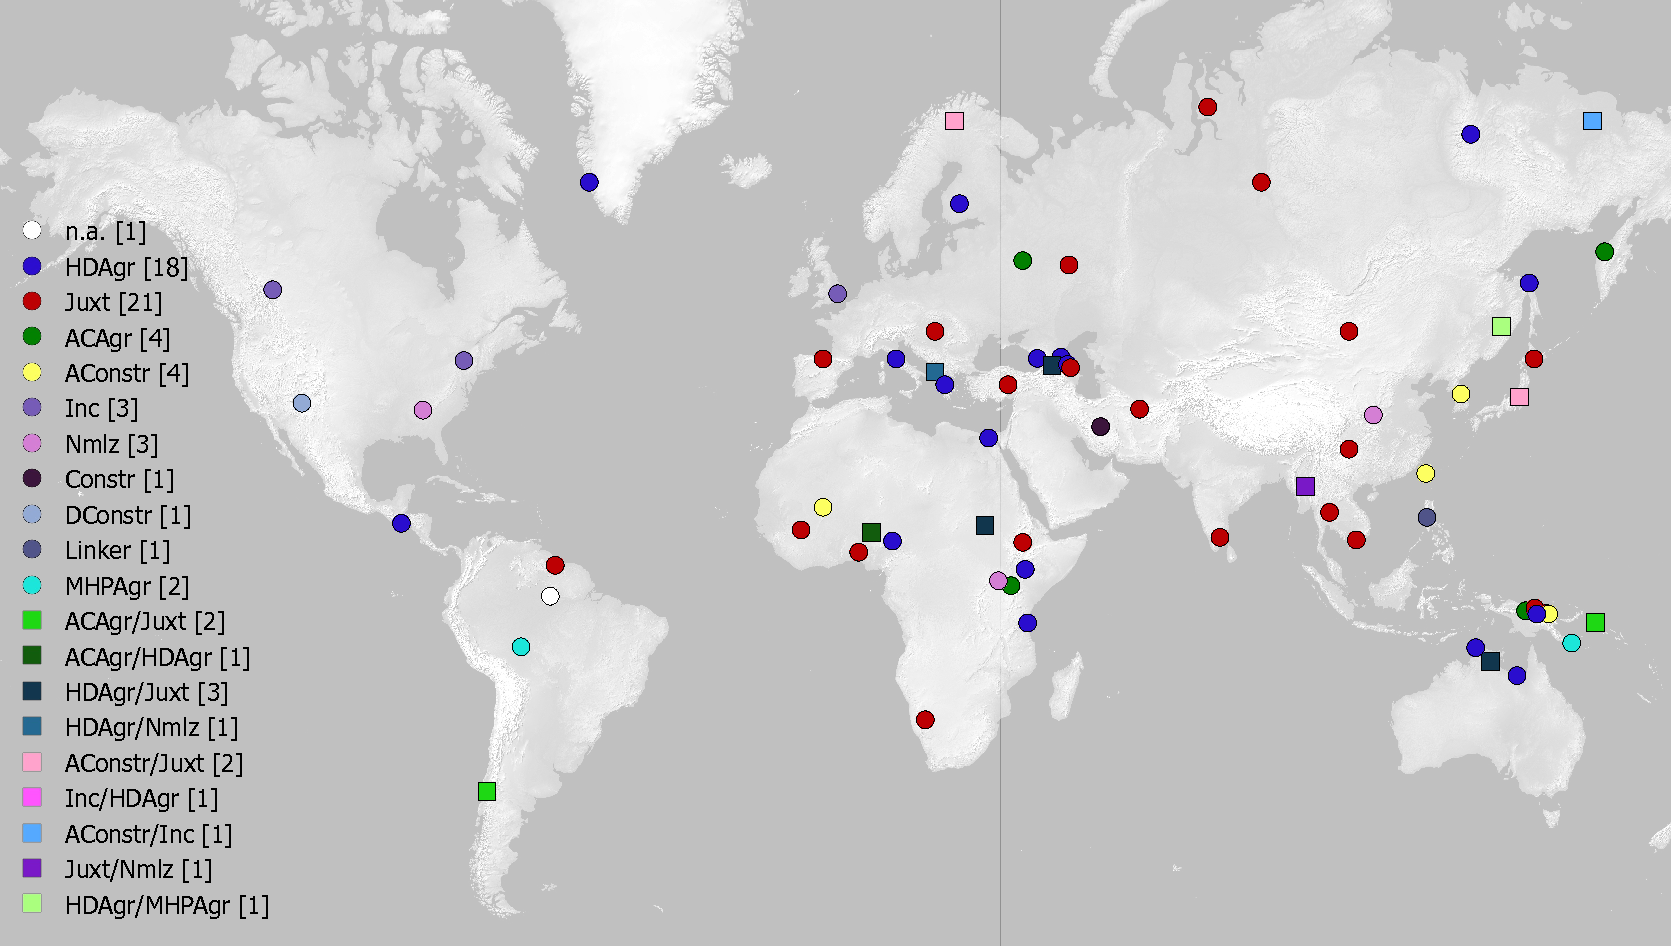
\includegraphics[width=\textwidth]{figures/WorldMap.pdf}
\label{WorldMap}
\end{sidewaysfigure}

\newpage
\begin{sidewaysfigure}
    
        \caption[Adjective attribution marking, World, main types]{Adjective attribution marking in the world's languages; (unbalanced) sample of 71 languages coded for main morpho-syntactic types}

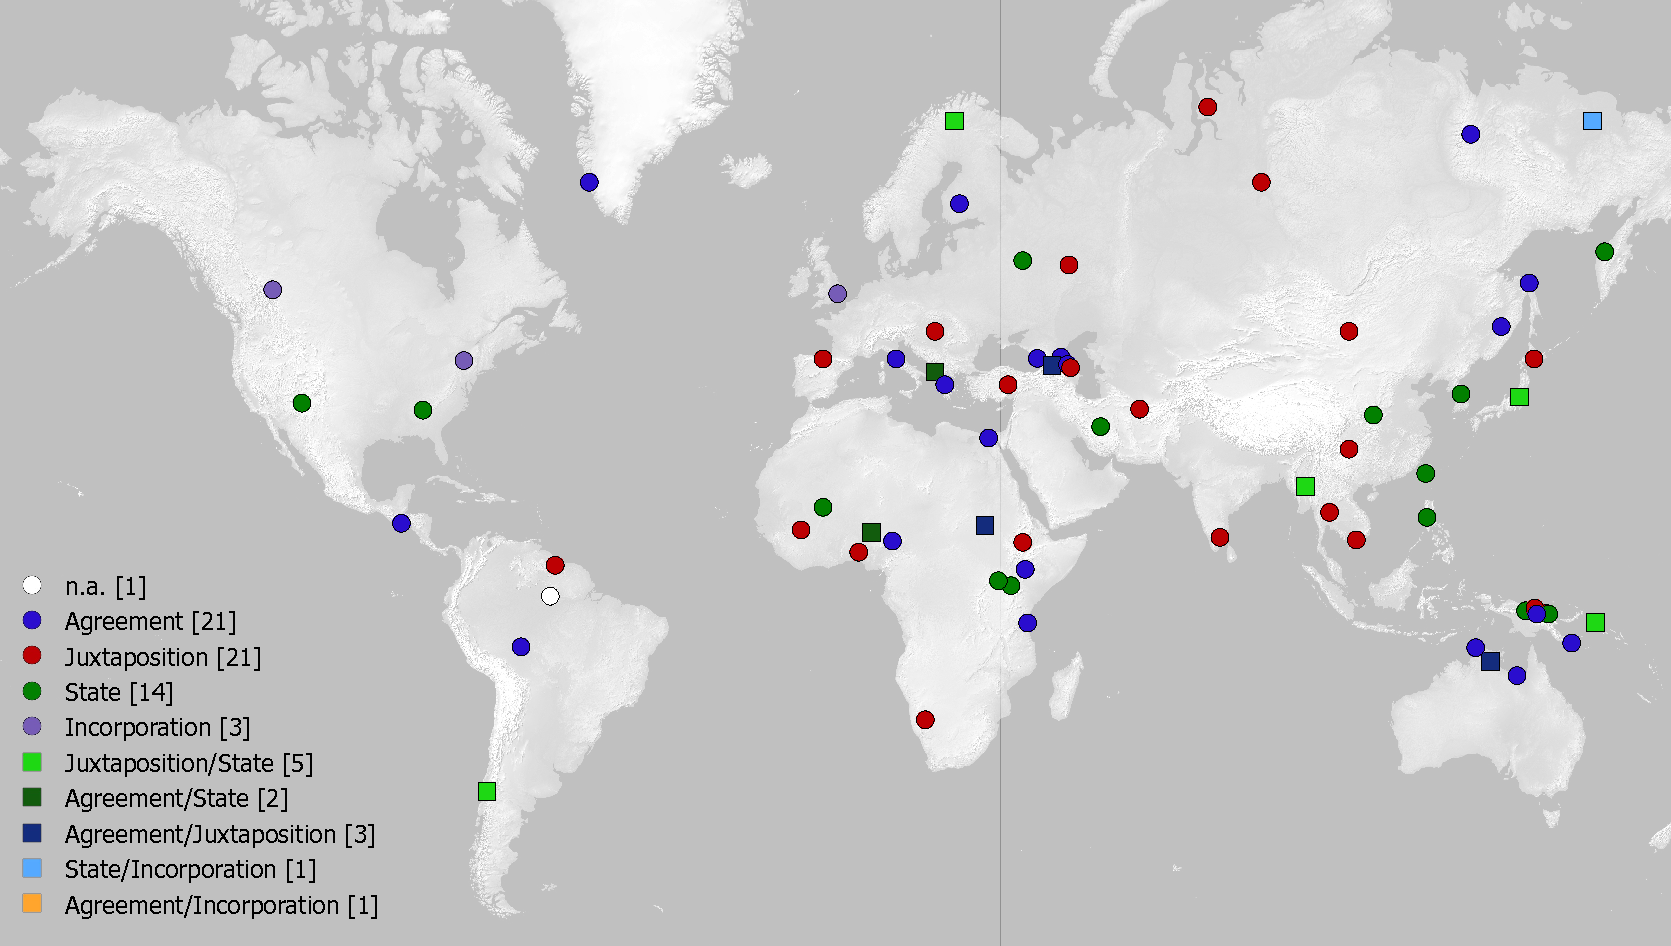
\includegraphics[width=\textwidth]{figures/WorldMapTyp.pdf}
\label{WorldMapTyp}
\end{sidewaysfigure}

\newpage
\begin{sidewaysfigure}
 \caption[Adjective attribution marking, North Eurasia]{Adjective attribution marking in the languages of North Eurasia; 90 languages representing all taxa of the area}
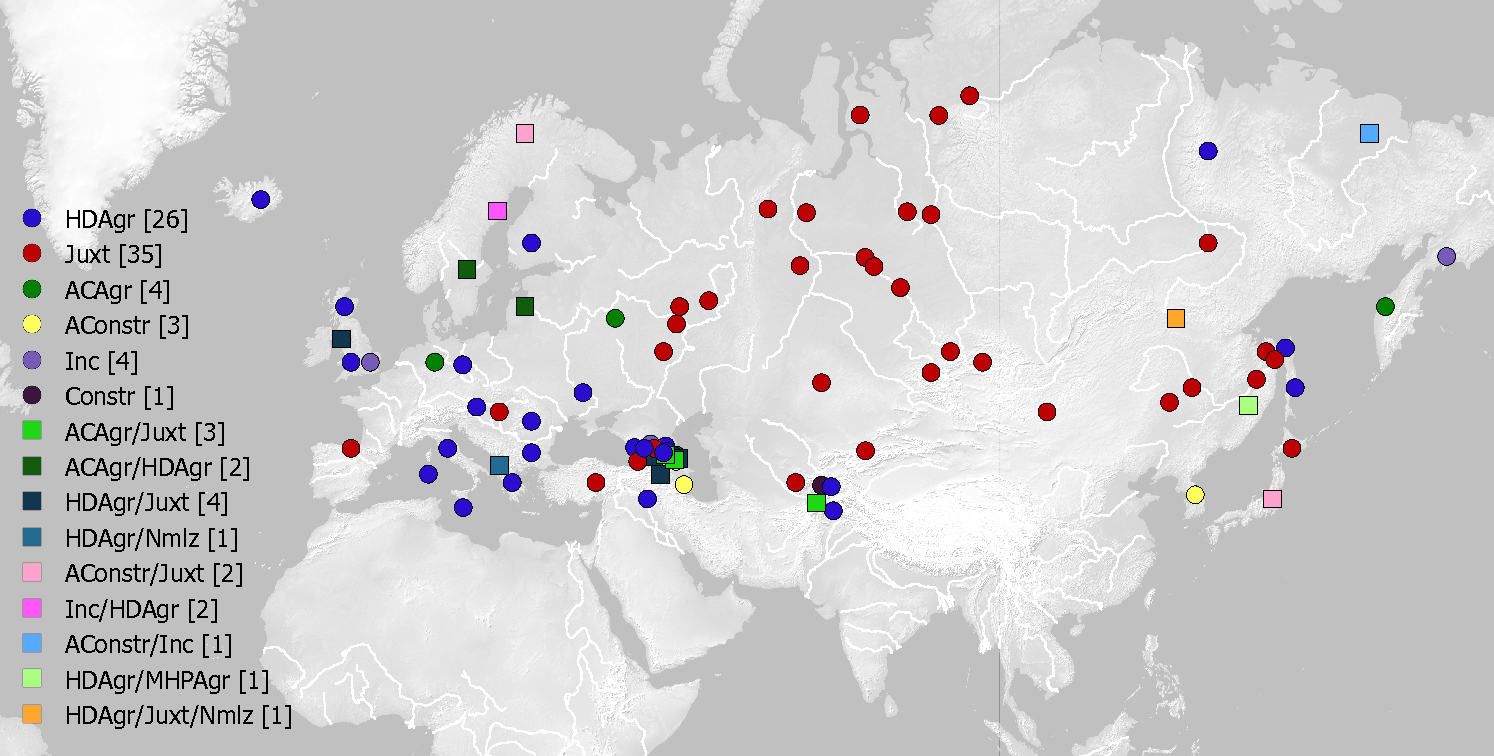
\includegraphics[width=\textwidth]{figures/NEMap.pdf}
\label{NEMap}
\end{sidewaysfigure}

\newpage
\begin{sidewaysfigure}
 \caption[Adjective attribution marking, North Eurasia, main types]{Adjective attribution marking in the languages of North Eurasia; 90 languages representing all taxa of the area coded for main morpho-syntactic types}
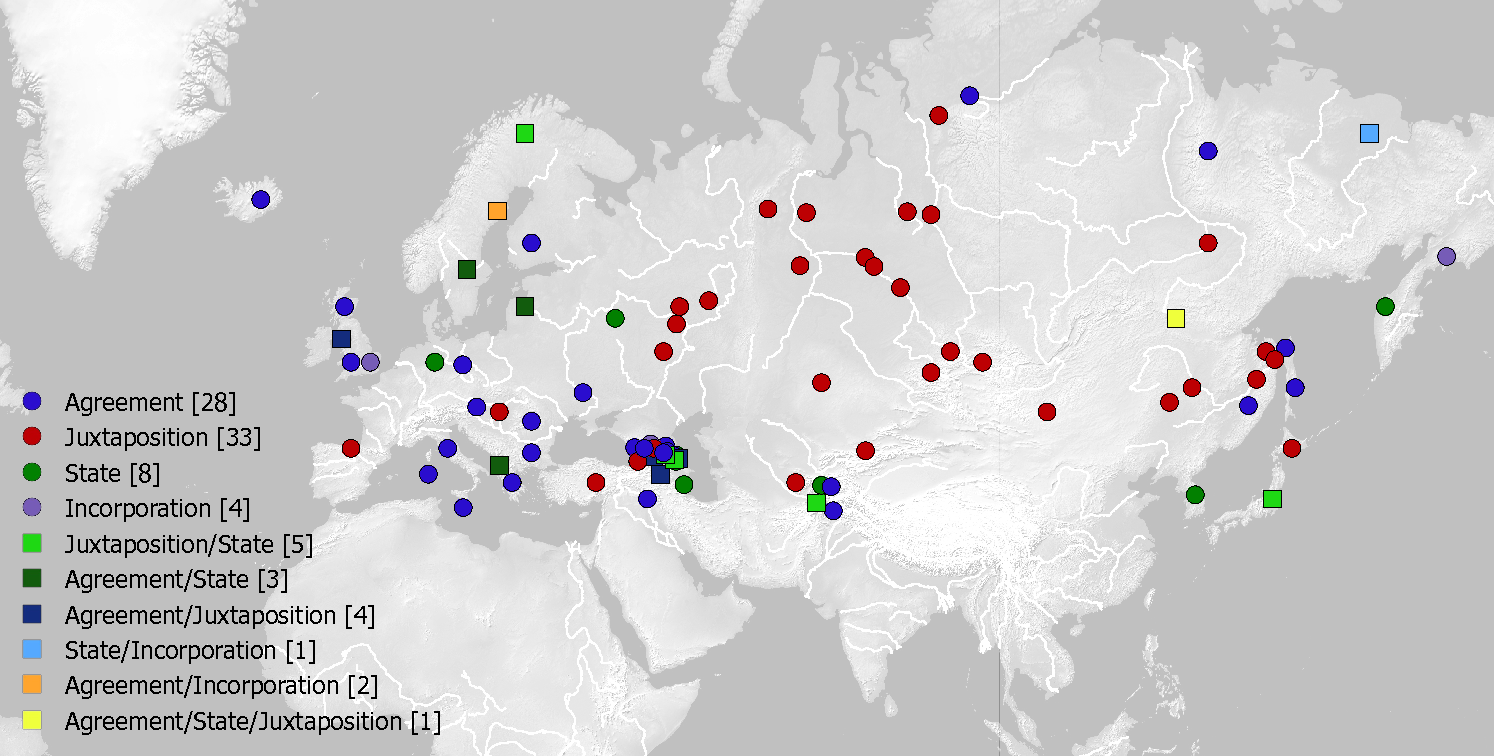
\includegraphics[width=\textwidth]{figures/NEMapTyp.pdf}
\label{NEMapTyp}
\end{sidewaysfigure}

\newpage
\begin{sidewaysfigure}
\caption[Adjective attribution marking, North Asia]{Adjective attribution marking in the languages of \isi{North Asia}; 58 languages}
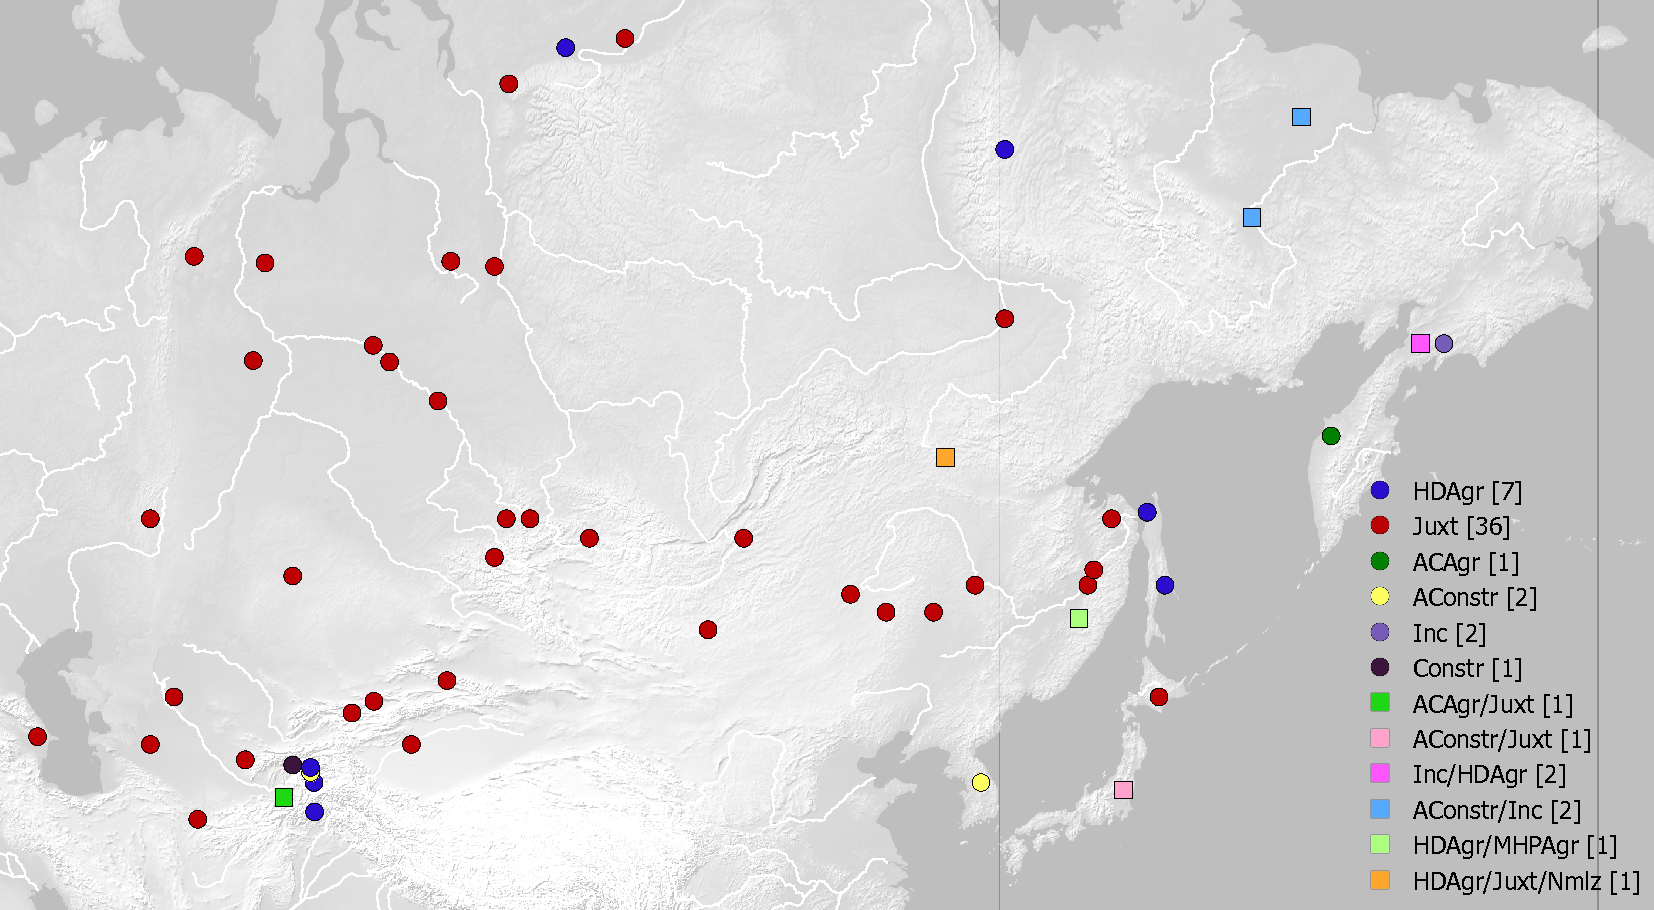
\includegraphics[width=\textwidth]{figures/NAMap.pdf}
\label{NAMap}
\end{sidewaysfigure}

\newpage
\begin{sidewaysfigure}
 \caption[Adjective attribution marking, North Asia, main types]{Adjective attribution marking in the languages of \isi{North Asia}; 58 languages coded for main morpho-syntactic types}
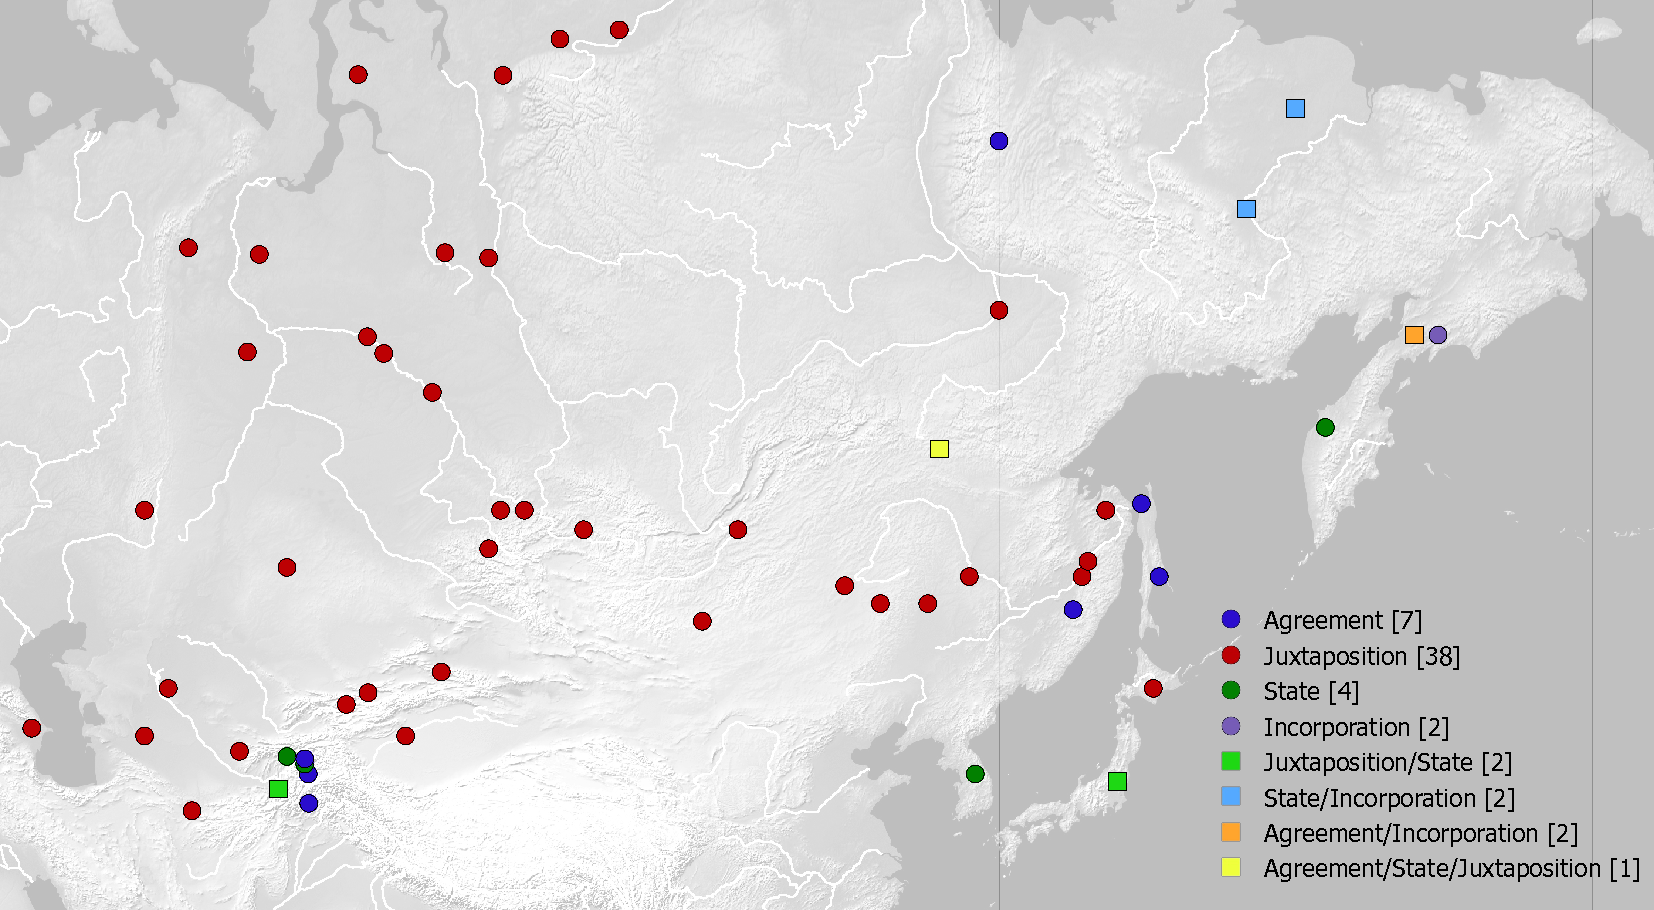
\includegraphics[width=\textwidth]{figures/NAMapTyp.pdf}
\label{NAMapTyp}
\end{sidewaysfigure}

\newpage
\begin{sidewaysfigure}
\caption[Adjective attribution marking, Europe]{Adjective attribution marking in the languages of \isi{Europe}; 123 languages}
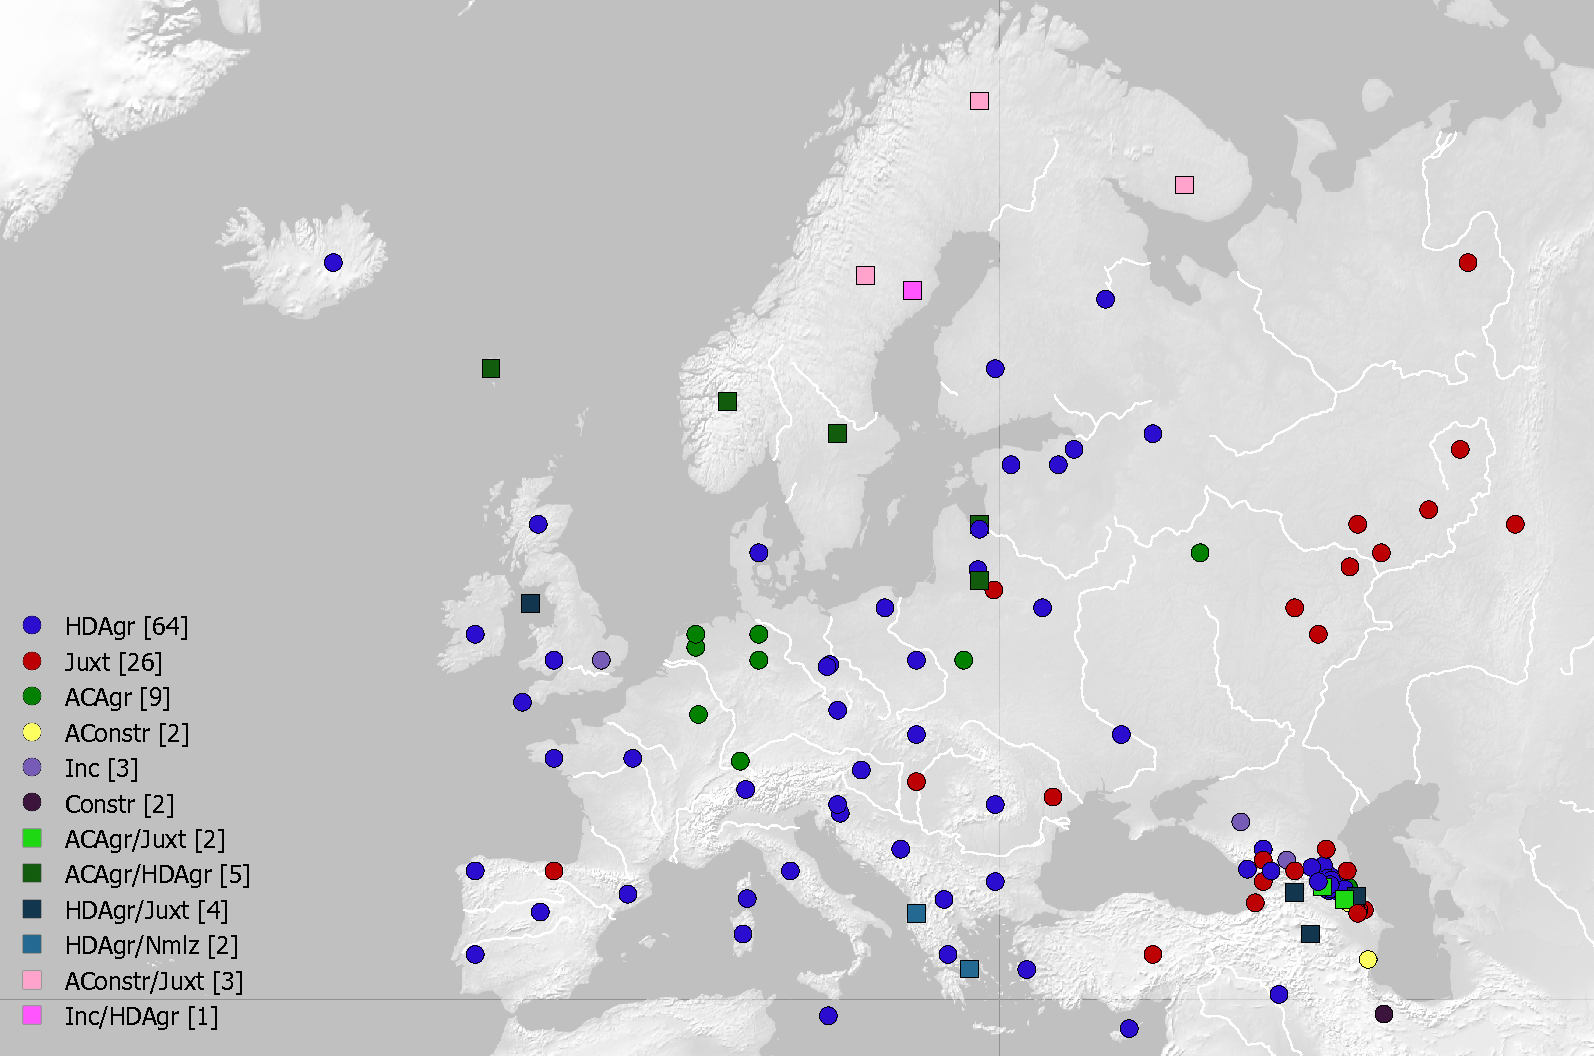
\includegraphics[width=\textwidth]{figures/EUMap.pdf}
\label{EUMap}
\end{sidewaysfigure}

\newpage
\begin{sidewaysfigure}
\caption[Adjective attribution marking, Europe, main types]{Adjective attribution marking in the languages of \isi{Europe}; 123 languages coded for main morpho-syntactic types}
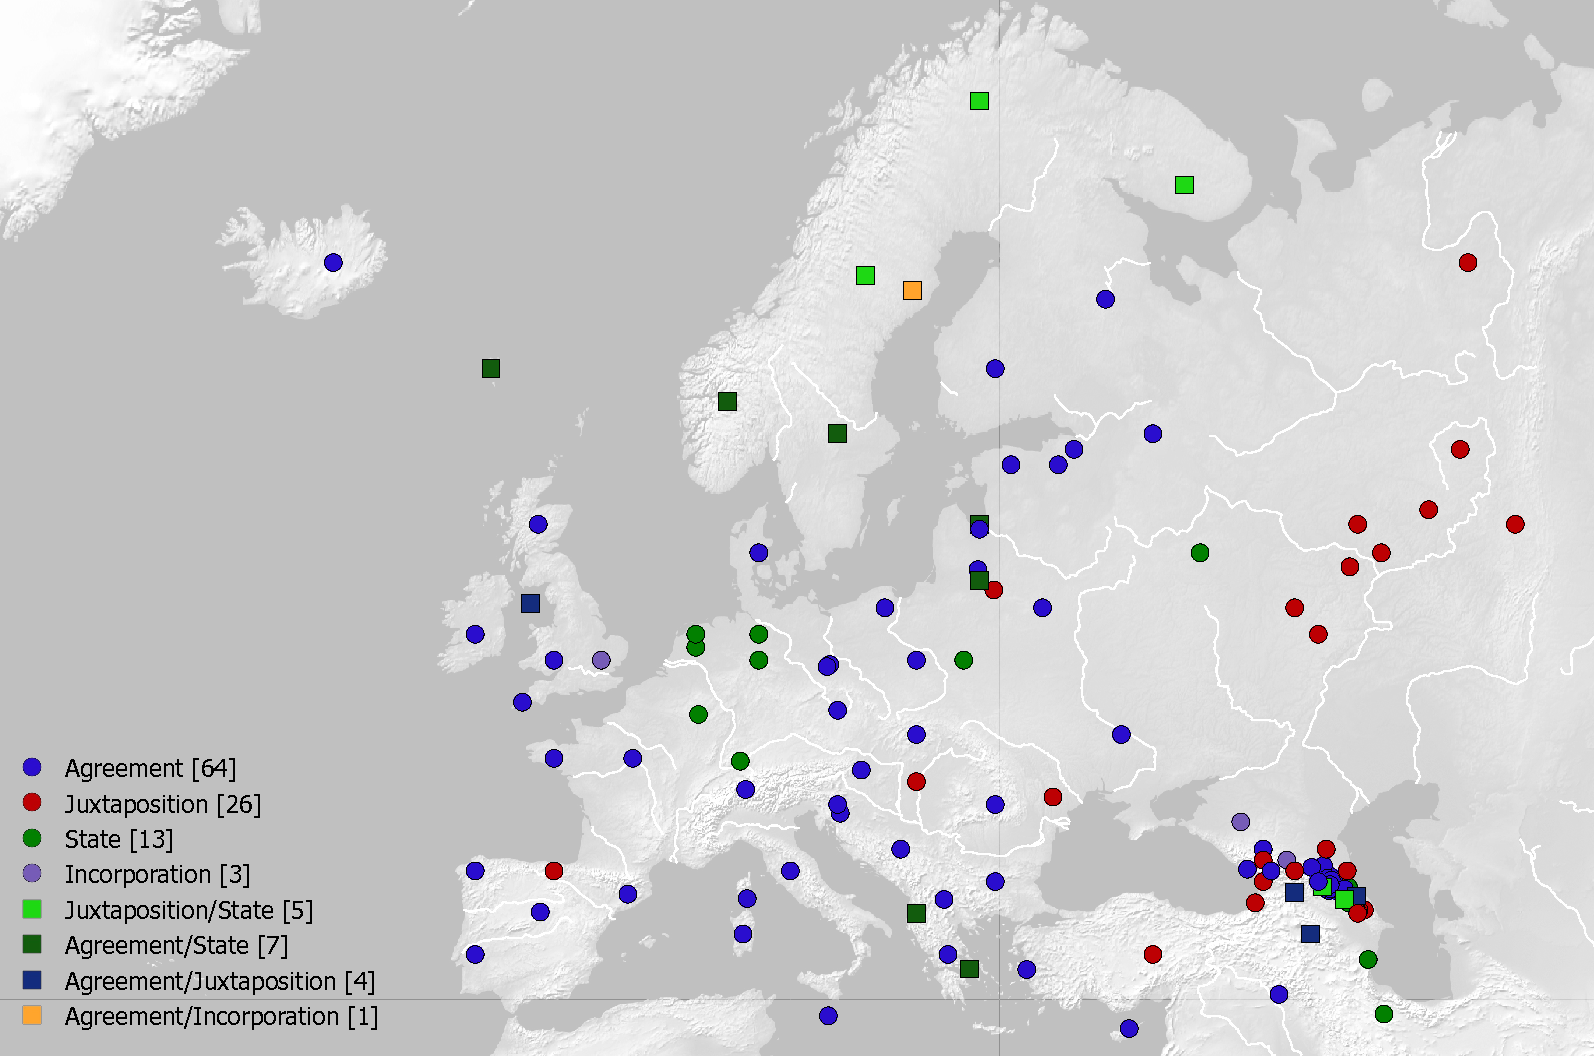
\includegraphics[width=\textwidth]{figures/EUMapTyp.pdf}
\label{EUMapTyp}
\end{sidewaysfigure}
